\section{Grundlagen}

\subsection[Ideologie des
Nationalsozialismus]{Ideologie\mycite[386\,--\,389]{gelbesGeschichts}
des Nationalsozialismus}
\index{Ideologie!Nationalsozialismus}
\index{Blut und Boden}
\index{Chauvinismus}
\index{Militarismus}

{
\small
\newlength{\antsemlength}
\settowidth{\antsemlength}{Antisemitismus}

\newcommand*{\nodebox}[1]{\parbox{\antsemlength}{#1}}

\begin{bundle}{\textbf{Sozialdarwinismus}}
  \chunk[\footnotesize Blut]{\nodebox{Rassismus\newline Antisemitismus}}
  \chunk[\footnotesize Boden]{
    \begin{bundle}{\nodebox{Nationalismus\newline \beg{Chauvinismus}}}
      \chunk{Führerprinzip}
      \chunk{Lebensraumtheorie}
      \chunk{Volksgemeinschaft}
      \chunk{Militarismus}
    \end{bundle}
  }
\end{bundle}
}


\subsubsection[Rassismus und Antisemitismus]{Rassismus und
Antisemitismus (siehe auch \ref{sec:aussch-gegner})}
\index{Rassismus}
\index{Antisemitismus}
\index{Rassenantisemitismus}
\index{Rassenlehre}
\index{Arier}

\begin{itemize}
\item Biologisierung des Sozialen -- Bestimmung des Verhaltens durch
Gene
\begin{itemize}
\item Höher-/Minderwertigkeit von Rassen: \jar{arische Rasse}
(nordisch), \jar{Kuli- und Fellachenrassen} (afrikanisch und
asiatisch), Juden
\item Schwache und Bedürftige schwächen mit ihren \jar{Erbanlagen} das
\jar{deutsche Volk}
\end{itemize}

\item Antisemitismus nicht mehr aus sozialen und religiösen Gründen,
sondern Rassenantisemitismus -- \jar{jüdische Rasse} als
\jar{minderwertig} und \jar{schmarotzend}

\item Rassismus und Antisemitismus werden zum Mittelpunkt des
politischen Denkens
\end{itemize}


\subsubsection{Führerkult}
\index{Führer}
\index{Führerkult}
\index{Führerprinzip}

\begin{itemize}
\item bedingungslose Unterwerfung des Einzelnen unter die Ziele des
Staates
\item Ausschluss von Opposition
\item Vereinigung aller Gewalten im \jar{Führer} 
\end{itemize}


\subsubsection{Lebensraumtheorie/-politik}
\index{Lebensraumtheorie}
\index{Lebensraumpolitik}

\begin{itemize}
\item \jar{germanische Rasse} hat Herrschaftsanspruch
\item Ausdehnung in Richtung Osten
\item Unterwerfung der \jar{Untermenschen}
\end{itemize}


\subsubsection{Volksgemeinschaftsideologie}
\index{Volksgemeinschaft}

\begin{itemize}
\item Wiedergeburt des deutschen Reiches
\item Verbot aller Parteien außer der NSDAP
\item Zusammenfassung aller politischen und sozialen Gruppen zu einer
\jar{Volksgemeinschaft}, Unterordnung und den Willen des \jar{Führers}
-- Überwindung sozialer, beruflicher und ideologischer Unterschiede
\end{itemize}


\subsection{Sicht des Großteils der Bevölkerung auf die Weimarer
Republik um 1933}

\begin{figure}
\centering
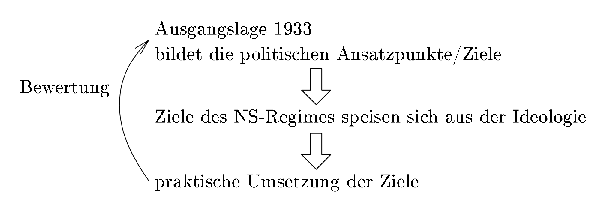
\includegraphics{bew-mass-ns.eps}
\caption{Bewertung der Wirksamkeit der Maßnahmen des NS-Regimes}
\label{pic:bew-mass-ns}
\end{figure}

Der Zustand der Weimarer Republik zu Anfang des Jahres 1933 bildete
die Ausgangslage für die Nationalsozialisten. Um deren Maßnahmen
hinsichtlich ihrer Wirksamkeit zu bewerten ist es zweckmäßig, zu
überprüfen, inwieweit sie Veränderungen gegenüber jener Ausgangslage
herbeiführten (siehe Abbildung \ref{pic:bew-mass-ns}) und wie die
Bevölkerung reagierte.

\begin{itemize}
\item wirtschaftliche Krise -- hohe Arbeitslosigkeit und Armut

\item Verhinderung wirtschaftlicher Erholung durch unfähige Demokraten
(\Nam{Brüning, Heinrich}{Brüning}s Deflationspolitik)

\item Wunsch nach
\begin{itemize}
\item Revision des \Ges{Vertrag von Versailles}{Vertrags von Versailles}

\item großdeutschem Reich -- Deutschland als militärische und
politische Großmacht

\item Verringerung der Arbeitslosigkeit
\end{itemize} 
\end{itemize}

%%%%%%%%%%%%%%%%%%%%%%%%%%%%%%%%%%%%%%%%%%%%%%%%%%%%%%%%%%%%%%%%%%%%%%

\subsection{Ziele der nationalsozialistischen Politik}

Aus dem vorhergehenden Abschnitt ergaben sich folgende Ansatzpunkte
für die Nationalsozialisten, um sich die Unterstützung der Bevölkerung
zu sichern:

\begin{itemize}
\item Wirtschaft
\begin{itemize}
\item Autarkie
\item Bekämpfung der Arbeitslosigkeit 
\end{itemize} 

\item Innenpolitik
\begin{itemize}
\item Ausschaltung der legalen Machtbasis
\item Zentralgewalt
\item Ausgrenzung der Nichtarier
\end{itemize}

\item Außenpolitik
\begin{itemize}
\item Revision des \Ges{Vertrag von Versailles}{Vertrags von Versailles}
\item Osterweiterung
\end{itemize}
\end{itemize}

Diese Ziele leiteten sich ebenfalls aus der Ideologie des
Nationalsozialismus ab, welche sich wiederum im \Ges{NSDAP,
Nationalsozialistische Deutsche Arbeiterpartei!Programm}{Programm der
NSDAP}\mycite{ProgNSDAP} niederschlug.

\endinput
